\section{事件的独立性}
\label{sec:cprob-independence}

不放回摸球时，第一个球的颜色改变了第二个球的概率：$\mathbb{P}(H_2\mid H_1)=1/2$，而$\mathbb{P}(H_2)=3/5$。放回摸球时，第一个球摸出后又放了回去，盒中构成不变，无论第一个是什么颜色，第二个是黑球的概率都是$3/5$。在后一种情形下，知道第一个结果不提供关于第二个结果的任何信息，计算交事件的概率时可以把两个概率直接相乘。怎样把“不提供信息”准确地写出来？

\paragraph{定义}
放回摸球的有序记录有$25$个等可能结果，其中两个都是黑球的有$3\times3=9$个，所以
\[
 \mathbb{P}(H_2\mid H_1)=\frac{9/25}{15/25}=\frac35=\mathbb{P}(H_2).
\]
条件概率等于原来的概率，就是“已知$H_1$不改变$H_2$的可能性”。把等式$\mathbb{P}(H_2\mid H_1)=\mathbb{P}(H_2)$乘以$\mathbb{P}(H_1)$，得到一个对两个事件对称的乘积形式，并且在条件事件概率为零时也有意义。

\begin{definition}[两个事件的独立]
\label{def:cprob-independent}
若事件$A,B$满足
\begin{equation}
 \mathbb{P}(A\cap B)=\mathbb{P}(A)\,\mathbb{P}(B),
 \label{eq:cprob-independent}
\end{equation}
就称$A$与$B$\term{独立}（independent）。
\end{definition}

当$\mathbb{P}(B)>0$时，由定义~\eqref{eq:cprob-conditional}，式~\eqref{eq:cprob-independent}等价于$\mathbb{P}(A\mid B)=\mathbb{P}(A)$；当$\mathbb{P}(A)>0$时，它也等价于$\mathbb{P}(B\mid A)=\mathbb{P}(B)$。所以独立是对称的：$B$不提供关于$A$的信息，$A$也不提供关于$B$的信息。

\paragraph{独立是数量关系}
独立性要按式~\eqref{eq:cprob-independent}核对，不能凭“看起来有没有关系”判断。从一副$52$张的牌中抽一张，令$A$为“抽到A”，$B$为“抽到红桃”。四张A中恰有一张红桃，所以
\[
 \mathbb{P}(A\cap B)=\frac{1}{52},\qquad
 \mathbb{P}(A)\,\mathbb{P}(B)=\frac{4}{52}\cdot\frac{13}{52}=\frac{1}{52}.
\]
二者独立。原因在于一副牌是$13$种点数与$4$种花色的全部搭配，每种点数在各花色中出现的比例都相同。

掷两枚骰子，令$A$为“第一枚是偶数”，$C$为“点数和为$7$”，$D$为“点数和为$8$”。点数和要用到第一枚的点数，似乎不会与$A$独立。在图~\ref{fig:cprob-independence-grid}(a)中数一数：$A$占$18$格，$C$的$6$格中有$3$格落在$A$里，所以
\[
 \mathbb{P}(A\cap C)=\frac{3}{36}=\frac12\cdot\frac16=\mathbb{P}(A)\,\mathbb{P}(C).
\]
$A$与$C$独立。原因是对第一枚的每个点数$i$，第二枚都恰有一个点数$7-i$使和为$7$，和为$7$的比例在每一列中都是$1/6$。

\begin{BookInlineFigure}
  \centering
  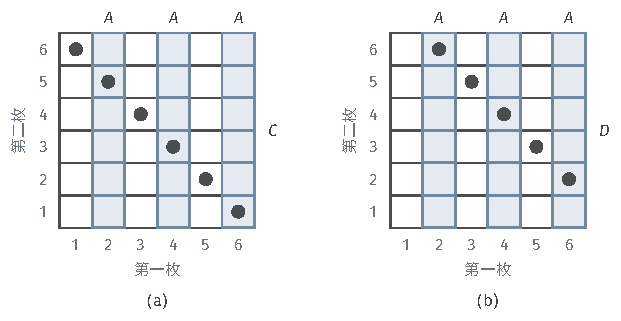
\includegraphics[width=105mm]{figures/07-probability/01-elementary-probability/tikz/cprob-independence-grid/figure.pdf}
  \caption{同一事件$A$（浅蓝三列，第一枚为偶数）与两个事件的关系。(a)圆点是$C$（点数和为$7$），在$A$内外各占所在列的$1/6$，$A$与$C$独立。(b)圆点是$D$（点数和为$8$），$A$内有$3$个、$A$外只有$2$个，$A$与$D$不独立。}
  \label{fig:cprob-independence-grid}
\end{BookInlineFigure}

$D$的情形不同。和为$8$的格子是$(2,6),(3,5),(4,4),(5,3),(6,2)$，其中第一枚为偶数的有$3$个，见图~\ref{fig:cprob-independence-grid}(b)。于是
\[
 \mathbb{P}(A\cap D)=\frac{3}{36},\qquad \mathbb{P}(A)\,\mathbb{P}(D)=\frac12\cdot\frac{5}{36}=\frac{2.5}{36}.
\]
两者不等，$A$与$D$不独立：第一枚为$1$时第二枚不可能凑出$8$，所以$D$在$A$之外的比例较低。对比$C$与$D$，事件之间在物理上是否“有关”不决定独立性，决定它的是交事件的比例。

\paragraph{独立与互斥}
互斥和独立都描述两个事件的关系，含义却几乎相反。互斥是集合之间的关系：$A\cap B=\varnothing$，两个事件不能同时发生，它与概率如何分配无关。独立是概率之间的关系：一个事件发生与否不改变另一个的概率，它取决于$\mathbb{P}$。

设$\mathbb{P}(A)>0$，$\mathbb{P}(B)>0$，且$A$与$B$互斥，则
\[
 \mathbb{P}(A\cap B)=0<\mathbb{P}(A)\,\mathbb{P}(B),
\]
二者不独立。这很合理：知道$B$发生，就确知$A$没有发生，$B$提供了关于$A$的完全信息。只有当其中一个事件的概率为零时，互斥的两个事件才独立。

\paragraph{补事件保持独立}
若$B$发生不提供关于$A$的信息，那么$B$不发生也不应提供信息。下面先对两个事件证实这一点，相互独立的多个事件在下一段定义之后再作推广。

\begin{theorem}[独立与补事件]
\label{thm:cprob-independent-complement}
若$A$与$B$独立，则$A$与$B^{\mathrm{c}}$独立，$A^{\mathrm{c}}$与$B$独立，$A^{\mathrm{c}}$与$B^{\mathrm{c}}$也独立。
\end{theorem}

\begin{proof}
$A$是互斥的$A\cap B$与$A\cap B^{\mathrm{c}}$之并，由互斥可加性与独立性，
\[
 \mathbb{P}(A\cap B^{\mathrm{c}})=\mathbb{P}(A)-\mathbb{P}(A\cap B)=\mathbb{P}(A)\bigl(1-\mathbb{P}(B)\bigr)=\mathbb{P}(A)\,\mathbb{P}(B^{\mathrm{c}}).
\]
所以$A$与$B^{\mathrm{c}}$独立。交换$A,B$的角色得到第二个结论；对独立的$A^{\mathrm{c}}$与$B$再用一次第一个结论，得到第三个。
\end{proof}

\paragraph{多个事件的相互独立}
三个或更多事件时，“互不提供信息”的要求更强：不仅任意两个之间不提供信息，任意几个事件的发生情况也不应改变其余事件的概率。这需要对所有子组都验证乘积关系。

\begin{definition}[相互独立]
\label{def:cprob-mutually-independent}
称事件$A_1,\ldots,A_n$\term{相互独立}（mutually independent），若对任意$2\leq k\leq n$和任意下标$1\leq i_1<\cdots<i_k\leq n$，都有
\begin{equation}
 \mathbb{P}(A_{i_1}\cap\cdots\cap A_{i_k})=\mathbb{P}(A_{i_1})\cdots\mathbb{P}(A_{i_k}).
 \label{eq:cprob-mutually-independent}
\end{equation}
若只要求$k=2$的情形，即任意两个事件独立，就称它们\term{两两独立}（pairwise independent）。
\end{definition}

两两独立不能推出相互独立。抛两枚均匀硬币，四个有序结果等可能。令$A$为“第一枚正面”，$B$为“第二枚正面”，$C$为“两枚结果相同”。每个事件的概率都是$1/2$；由图~\ref{fig:cprob-two-coins-pairwise}，任意两个事件恰好共有一个结果，所以每对的交的概率都是$1/4=(1/2)^2$，三对都独立。

\begin{BookInlineFigure}
  \centering
  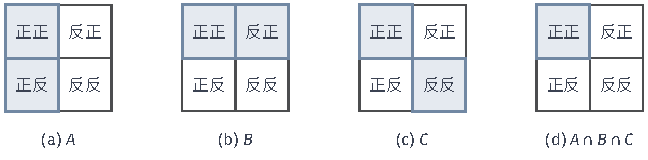
\includegraphics[width=110mm]{figures/07-probability/01-elementary-probability/tikz/cprob-two-coins-pairwise/figure.pdf}
  \caption{抛两枚硬币的四个等可能结果，“正反”表示第一枚正面、第二枚反面。浅蓝格子依次是(a)$A$：第一枚正面；(b)$B$：第二枚正面；(c)$C$：两枚相同；(d)$A\cap B\cap C$。任意两个事件的交都只有“正正”一格，三者之交也只有这一格。}
  \label{fig:cprob-two-coins-pairwise}
\end{BookInlineFigure}

但三个事件同时发生就是“正正”，于是
\[
 \mathbb{P}(A\cap B\cap C)=\frac14\neq\frac18=\mathbb{P}(A)\,\mathbb{P}(B)\,\mathbb{P}(C).
\]
三者不相互独立。原因很清楚：知道$A$与$B$都发生，就完全知道了$C$；单独知道其中任何一个，却对另一个毫无帮助。

反过来，只验证三者之交的乘积关系也不够。掷两枚骰子，令$E_1$为“第一枚是$1,2,3$之一”，$E_2$为“第一枚是$3,4,5$之一”，$E_3$为“点数和为$9$”。$E_1\cap E_2\cap E_3$只有结果$(3,6)$，于是
\[
 \mathbb{P}(E_1\cap E_2\cap E_3)=\frac{1}{36}=\frac12\cdot\frac12\cdot\frac19.
\]
然而$E_1\cap E_2$是“第一枚是$3$”，概率$1/6\neq1/4$，这两个事件不独立。定义~\ref{def:cprob-mutually-independent}要求所有子组的乘积关系，任何一层都不能省略。

\paragraph{多个事件的补}
定理~\ref{thm:cprob-independent-complement}可以推广到相互独立的多个事件：把其中任意几个换成补事件，所得的事件仍相互独立。只需说明换掉一个即可，换多个时逐个替换。设$A_1,\ldots,A_n$相互独立，把$A_1$换成$A_1^{\mathrm{c}}$。对含下标$1$的子组，记其余事件之交为$F$。由于$A_1,\ldots,A_n$的乘积关系对每个子组成立，$\mathbb{P}(F)$等于其余各事件概率之积，并且
\[
 \mathbb{P}(A_1\cap F)=\mathbb{P}(A_1)\,\mathbb{P}(F).
\]
重复定理~\ref{thm:cprob-independent-complement}的证明，得到
\[
 \mathbb{P}(A_1^{\mathrm{c}}\cap F)=\mathbb{P}(F)-\mathbb{P}(A_1\cap F)=\mathbb{P}(A_1^{\mathrm{c}})\,\mathbb{P}(F).
\]
不含下标$1$的子组不受影响，所以式~\eqref{eq:cprob-mutually-independent}对新的一组事件仍成立。

\paragraph{重复试验中的独立性从哪里来}
“两次投掷互不影响”这句话，在模型中究竟对应什么？以两枚骰子为例，样本空间是乘积$\Omega=\Omega_1\times\Omega_2$，$\Omega_1=\Omega_2=\{1,\ldots,6\}$，第~\ref{sec:cprob-equally-likely}节假设这$36$个有序对同样可能。只与第一枚有关的事件形如$A_1\times\Omega_2$，只与第二枚有关的事件形如$\Omega_1\times A_2$，它们的交是矩形$A_1\times A_2$，如图~\ref{fig:cprob-product-space}所示。

\begin{BookInlineFigure}
  \centering
  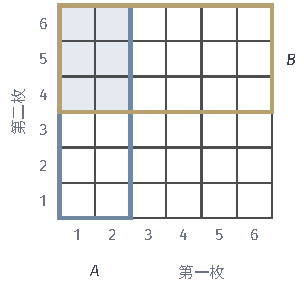
\includegraphics[width=53mm]{figures/07-probability/01-elementary-probability/tikz/cprob-product-space/figure.pdf}
  \caption{乘积样本空间中的独立性。蓝框是$A$：第一枚为$1$或$2$；黄框是$B$：第二枚为$4,5,6$之一。交$A\cap B$是$2\times3$的浅蓝矩形，其格数等于两边格数之积。}
  \label{fig:cprob-product-space}
\end{BookInlineFigure}

\begin{theorem}[乘积样本空间上的独立性]
\label{thm:cprob-product-independence}
设$\Omega=\Omega_1\times\cdots\times\Omega_n$，各$\Omega_k$有限且非空，$\Omega$上的全部结果同样可能。对每个$k$取$A_k\subseteq\Omega_k$，令
\begin{equation}
 E_k=\{(\omega_1,\ldots,\omega_n)\in\Omega:\ \omega_k\in A_k\}
 \label{eq:cprob-coordinate-event}
\end{equation}
为只与第$k$个分量有关的事件。则$E_1,\ldots,E_n$相互独立，并且
\begin{equation}
 \mathbb{P}(E_k)=\frac{\lvert A_k\rvert}{\lvert\Omega_k\rvert}.
 \label{eq:cprob-product-marginal}
\end{equation}
\end{theorem}

\begin{proof}
任取下标集合$S\subseteq\{1,\ldots,n\}$。按式~\eqref{eq:cprob-coordinate-event}，$\bigcap_{k\in S}E_k$由第$k$个分量在$A_k$中（$k\in S$）、其余分量任意的结果组成，它是乘积集合，各分量的取值范围分别是$A_k$（$k\in S$）或$\Omega_k$（$k\notin S$）。由乘法规则计数，
\[
 \Bigl\lvert\bigcap_{k\in S}E_k\Bigr\rvert=\prod_{k\in S}\lvert A_k\rvert\prod_{k\notin S}\lvert\Omega_k\rvert.
\]
$\Omega$本身也是乘积集合，$\lvert\Omega\rvert$等于各$\lvert\Omega_k\rvert$之积。两式相除，得到
\[
 \mathbb{P}\Bigl(\bigcap_{k\in S}E_k\Bigr)=\prod_{k\in S}\frac{\lvert A_k\rvert}{\lvert\Omega_k\rvert}.
\]
取$S=\{k\}$即得式~\eqref{eq:cprob-product-marginal}；把它代回上式，对每个至少含两个下标的$S$都得到式~\eqref{eq:cprob-mutually-independent}。
\end{proof}

定理说明，重复试验中的独立性是乘积样本空间上等可能假设的推论。这个假设比“每次试验各自等可能”更多：它还要求各次结果的每种搭配同样可能，这正是“互不影响”在模型中的含义。放回摸球的$25$个有序对是$\{1,\ldots,5\}\times\{1,\ldots,5\}$的全部，满足定理的条件，所以$H_1$与$H_2$独立。

不放回摸球的样本空间去掉了对角线，不再是乘积集合，定理不适用；实际计算也表明$\mathbb{P}(H_1\cap H_2)=3/10$，而$\mathbb{P}(H_1)\,\mathbb{P}(H_2)=9/25$，二者不独立。每一次单独看，第二个球在五个球中仍是等可能的，$\mathbb{P}(H_2)=3/5$；不独立来自两次之间的搭配受到限制。

\paragraph{至少成功一次}
独立性使“$n$次重复中至少成功一次”的计算变得简单。设每次试验中某事件发生的概率为$p$，各次的事件相互独立。由上面关于补事件的推广，各次“不发生”的事件也相互独立，所以$n$次都不发生的概率是$(1-p)^{n}$，于是
\begin{equation}
 \mathbb{P}(\text{至少发生一次})=1-(1-p)^{n}.
 \label{eq:cprob-at-least-once}
\end{equation}

一个经典的比较是：掷一枚骰子$4$次至少出现一个六点，与掷两枚骰子$24$次至少出现一次双六，哪个更可能？前者$p=1/6$，后者$p=1/36$，由式~\eqref{eq:cprob-at-least-once}，
\[
 1-\Bigl(\frac56\Bigr)^{4}\approx0.5177,\qquad
 1-\Bigl(\frac{35}{36}\Bigr)^{24}\approx0.4914.
\]
虽然$4/6=24/36$，两者却一个略大于一半、一个略小于一半。图~\ref{fig:cprob-repeated-trials}画出两条曲线：概率不是随次数线性增长，而是以$1-(1-p)^{n}$的形式逐渐接近$1$，“机会乘以次数”只在$np$很小时近似成立。

\begin{BookInlineFigure}
  \centering
  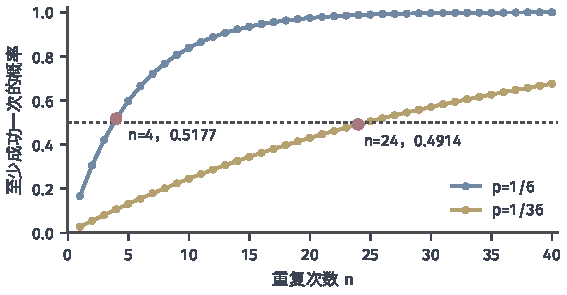
\includegraphics[width=96mm]{figures/07-probability/01-elementary-probability/matplotlib/cprob-repeated-trials/figure.pdf}
  \caption{$n$次独立重复中至少成功一次的概率$1-(1-p)^{n}$。蓝线$p=1/6$（一枚骰子出六点），黄线$p=1/36$（两枚骰子出双六），黑色点线是$1/2$；红点标出$n=4$与$n=24$两个值。}
  \label{fig:cprob-repeated-trials}
\end{BookInlineFigure}

同样的论证给出：$n$次中指定的$k$次成功、其余失败的概率是$p^{k}(1-p)^{n-k}$。在古典模型中$p$只能是有理数，例如$1/6$；成功次数的完整分布以及一般的$p$在第~\ref{chap:common-distributions}章讨论。

\paragraph{条件之下的独立}
回到第~\ref{sec:cprob-total-bayes}节的复检。那里假设的是：对次品，两次检测是否报警互不影响；对合格品也是如此。用本节的语言，就是$T_1$与$T_2$在条件概率$\mathbb{P}(\cdot\mid D)$下独立，在$\mathbb{P}(\cdot\mid D^{\mathrm{c}})$下也独立：
\[
 \mathbb{P}(T_1\cap T_2\mid D)=0.95^{2},\qquad
 \mathbb{P}(T_1\cap T_2\mid D^{\mathrm{c}})=0.05^{2}.
\]

不按状态区分时，$T_1$与$T_2$并不独立。由全概率公式，
\[
 \mathbb{P}(T_1\cap T_2)=0.02\times0.9025+0.98\times0.0025=0.0205,
\]
而两次报警各自的概率都是$0.068$，乘积为
\[
 \mathbb{P}(T_1)\,\mathbb{P}(T_2)=0.068^{2}\approx0.0046.
\]第一次报警提高了产品是次品的可能性，从而提高了第二次报警的可能性，两次报警通过产品的状态联系在一起。条件之下的独立与不加条件的独立是两回事，一般理论在第~\ref{chap:conditional-distributions}章建立。
